\chapter{Automatic Graphic User Interface Generator (AGG)}
	\label{sec:AGG}
	
	En este capítulo se presentan los motivos que llevaron a desarrollar una herramienta para generar en forma automática interfaces gráficas de usuario adaptadas a cada topología ferroviaria, así como también las bibliotecas de código utilizadas, las estrategias de comunicación y el diseño realizado.
	
	\section{Necesidad de contar con una herramienta para generar interfaces gráficas}
	
	La complejidad del sistema implementado en la FPGA en base al código generado por parte del ACG es tal que se vuelve indispensable contar con una herramienta gráfica que facilite la interpretación de los resultados. A su vez, es importante contar con una herramienta que pueda establecer la comunicación con la FPGA, tanto para enviar cómo para recibir las tramas de mensajes definida en la Sección \ref{sec:UART}. Para lograr estos objetivos se creó el AGG (del inglés, Automatic Graphic User Interface Generator), una herramienta diseñada e implementada por el autor de esta tesis de doctorado. El AGG permite establecer la comunicación con la FPGA y actualizar en tiempo real el estado de una interfaz gráfica basada en railML, intuitiva y a semejanza de una consola de señalamiento real.
	
	La interfaz de usuario generada por el AGG tiene como objetivo reemplazar a la mesa de señalamiento que se utiliza habitualmente para comandar los sistemas de enclavamiento en Argentina. En la Figura \ref{fig:enclavamiento_3} se presentó una foto de una mesa de enclavamientos real, y para comodidad del lector se muestra nuevamente esa foto en la Figura \ref{fig:enclavamiento_3_nueva}.
	
	\begin{figure}[H]
		\centering
		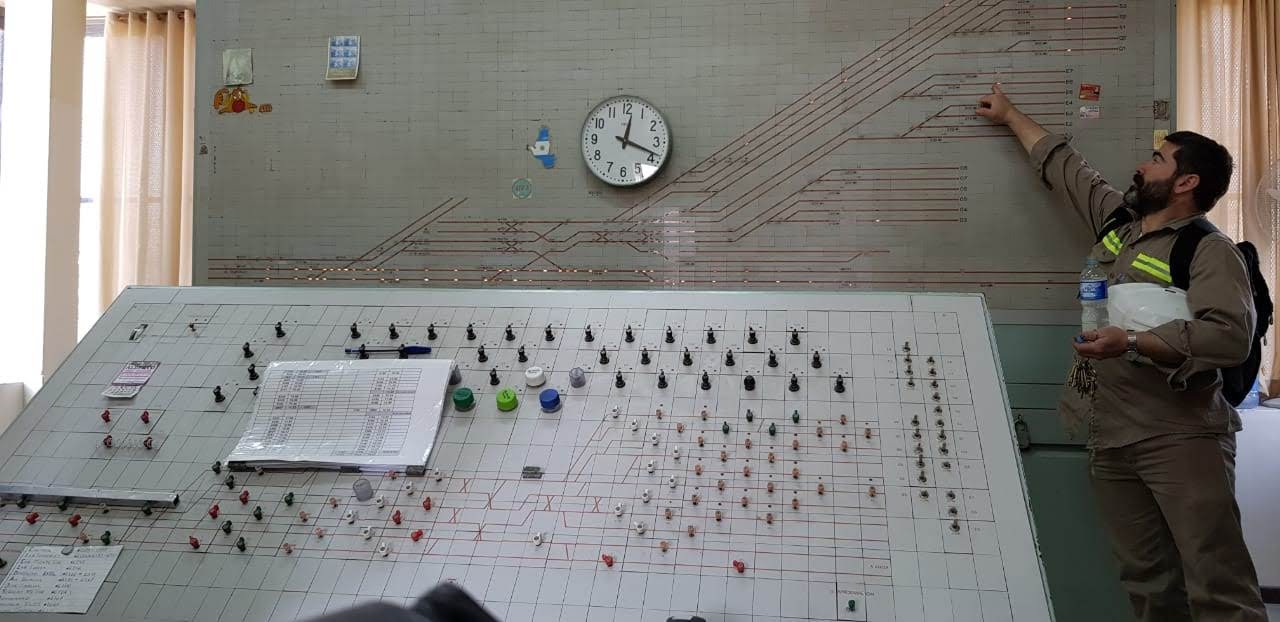
\includegraphics[width=1\textwidth]{Figuras/llavallol.jpg}
		\centering\caption{Panel de control central de un sistema de enclavamientos.}
		\label{fig:enclavamiento_3_nueva}
	\end{figure}
	
	\section{Diseño de la herramienta para la generación automática de interfaces de usuario}
	\label{sec:AGG_rutas}
	
	Para implementar el AGG se decidió utilizar la biblioteca tkinter \cite{TKINTER} para la interfaz gráfica de usuario y la biblioteca serial, nativa de Python, para establecer la comunicación con la plataforma FPGA. Ambas bibliotecas son las mas utilizadas debido a su amplia difusión en la comunidad de software libre, funcionalidades incluidas y detallada documentación.
	
	La interfaz gráfica se genera utilizando la información provista por el RNA (ver Sección \ref{sec:Biblioteca}), como por ejemplo la topología (posición, conexión y largo de las vías), la distribución de la infraestructura estática (plataformas, final de vías), la disposición de la infraestructura dinámica (cambios de vías, pasos a nivel) y el señalamiento (posición y orientación de las señales). El estado de la interfaz gráfica se actualiza en tiempo real y es reportado a la FPGA en una trama de datos, que ya fue explicada en la Sección \ref{sec:UART}.
	
	El usuario u operario puede interactuar con la interfaz creada mediante tres acciones: hacer zoom in/out utilizando la rueda del mouse, arrastrar la topología mientras se mantiene presionada la tecla shift para desplazarse por la interfaz y modificar el estado de los elementos de la interfaz que son interactivos al hacer click con el mouse sobre ellos. Los elementos interactivos son por ejemplo un cambio de vías, un paso a nivel o una vía. Los finales de vías no poseen estados y, por lo tanto, no son interactivos. Las tres acciones fueron implementadas en Python por el autor de esta tesis de doctorado mediante interrupciones, para tener una respuesta lo más cercana posible a tiempo real. 
	
	Las interacciones producto de hacer click sobre los elementos de la interfaz se dividen en dos tipos de eventos: estáticos y dinámicos. Un evento estático involucra al usuario que modifica el estado de la infraestructura, por ejemplo: ocupa o libera una vía, cierra o abre un paso a nivel o modifica la posición de un cambio de vías. Un evento dinámico implica la solicitud y cancelación de rutas. Todas estas acciones se pueden realizar con un click sobre el elemento que se desea modificar. El AGG informará a la FPGA del nuevo estado del elemento seleccionado y actualizará el color y/o posición del elemento, en base a la respuesta de la FPGA. 
	
	\section{Representación de cada elemento ferroviario en la interfaz gráfica}
	\label{sec:AGG_STATUS}
	
	Cada uno de los elementos ferroviarios presentes en la interfaz gráfica que son interactivos presentan diferentes formas y colores para representar sus estados. Por ejemplo, las tramos de vías definidos por la clase \textit{netElement} son ilustrados en la Figura \ref{fig:AGG_tracks}. La vía libre es representada de color negro, la vía ocupada por un tren es de color rojo, mientras que la vía que se encuentra enclavada por una ruta y no puede ser utilizada por ninguna otra formación, salvo la habilitada por esa ruta, se representa de color gris. El usuario podrá hacer click en cualquier parte de la vía, siendo mas notorios los límites en el caso de la vía roja o gris.
		
	\begin{figure}[H]
		\centering
		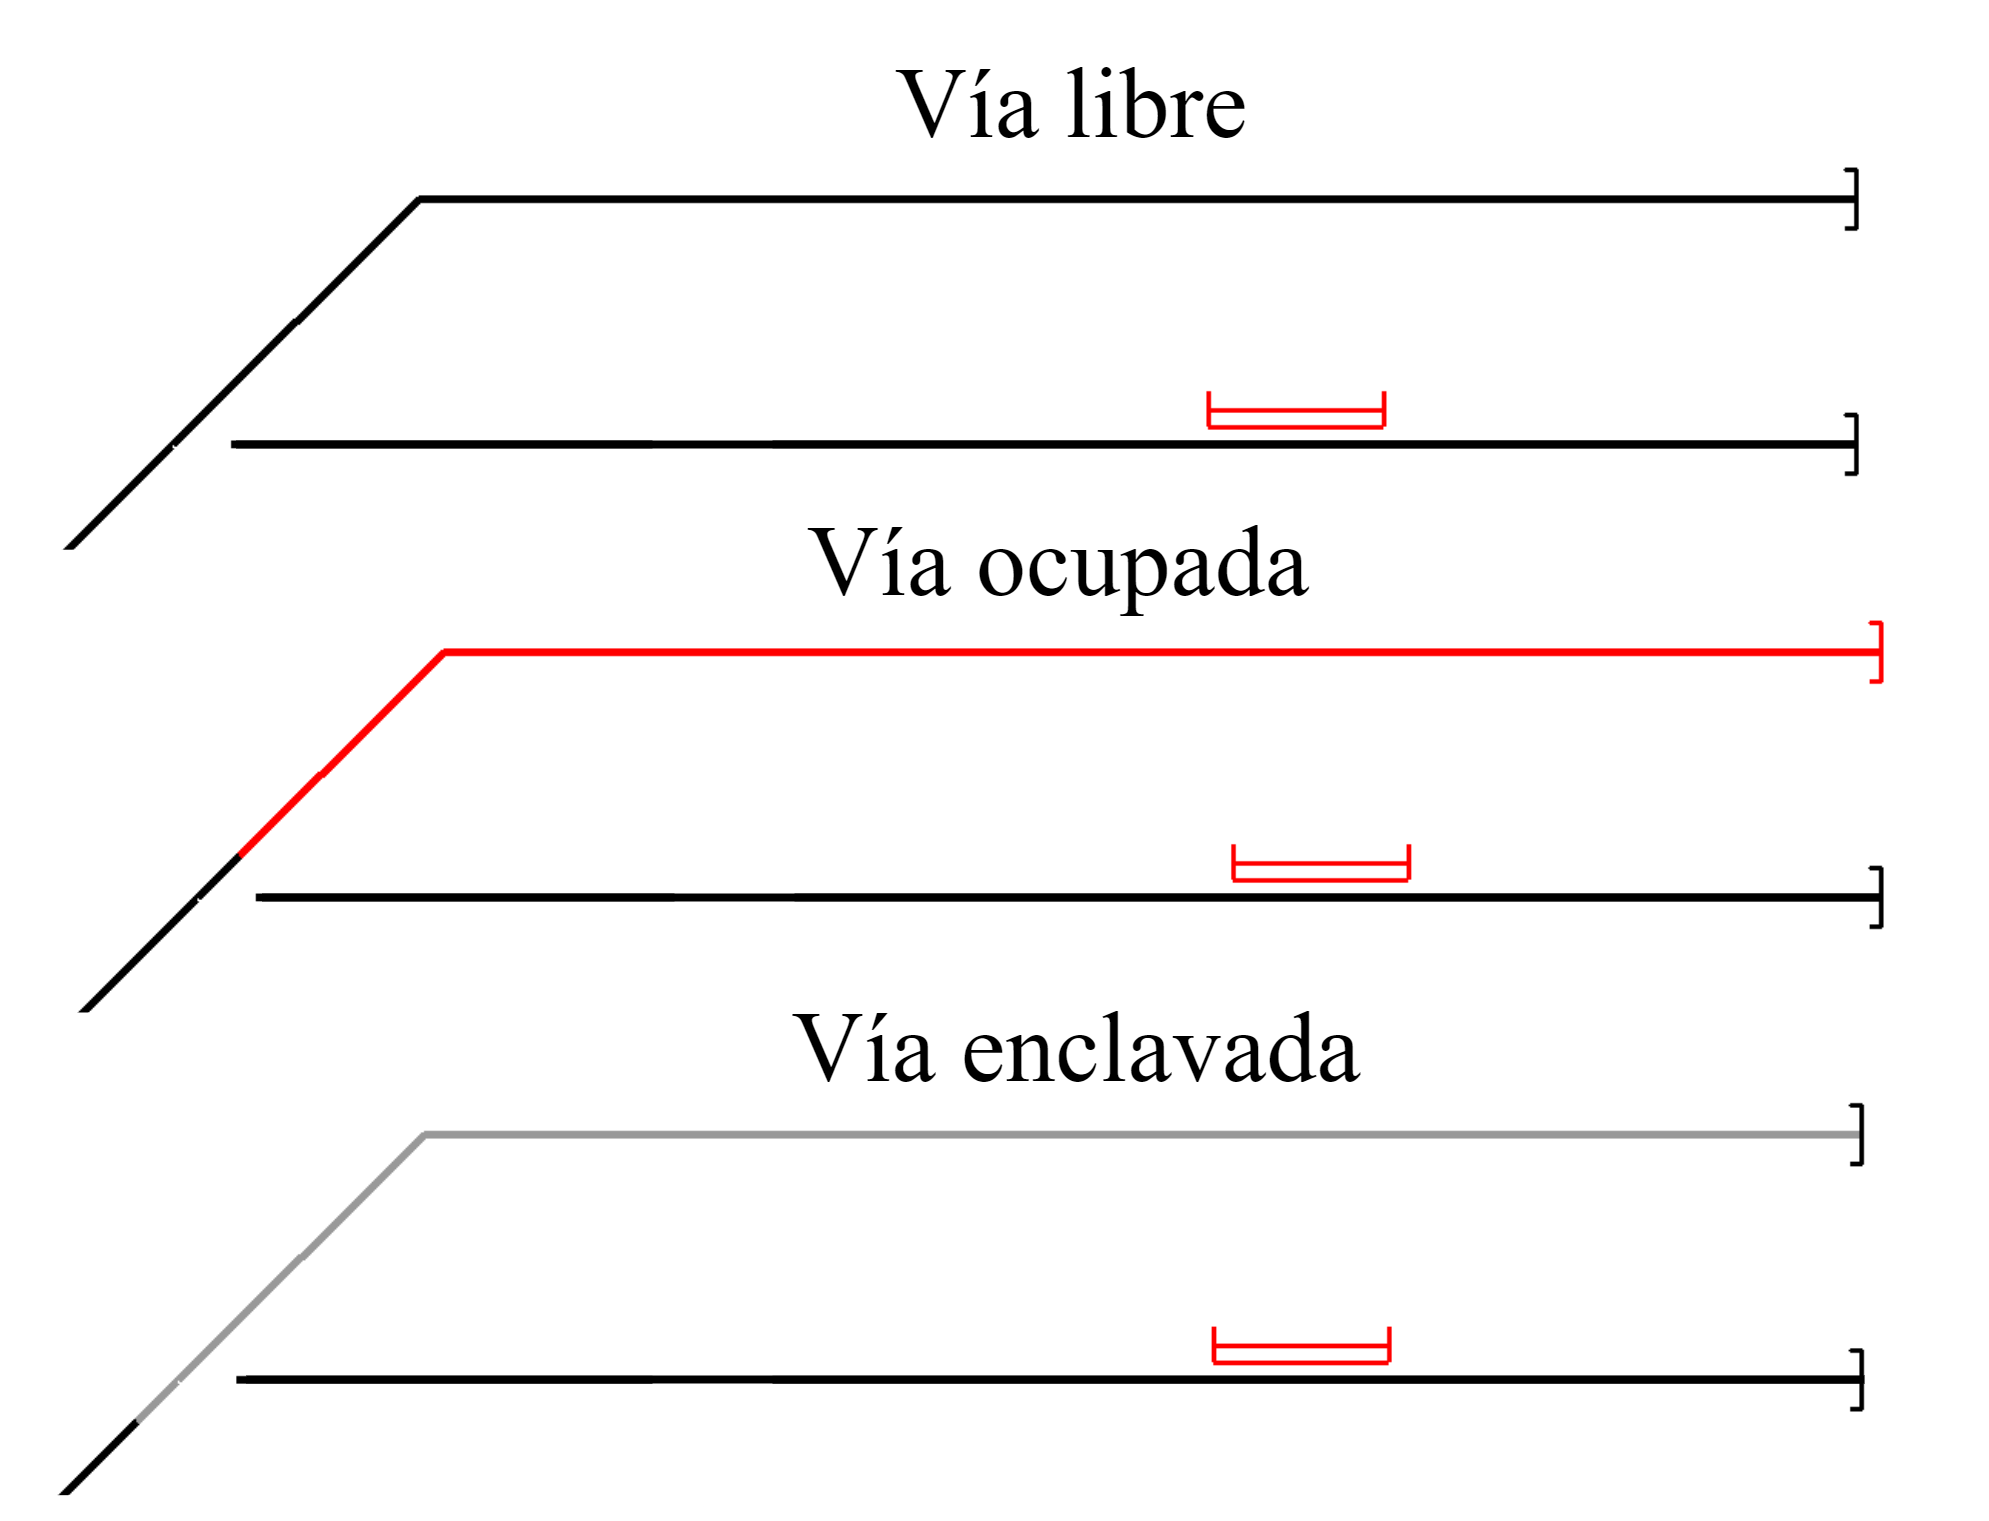
\includegraphics[width=0.7\textwidth]{AGG/images/AGG_via}
		\centering\caption{Representación de vía libre (arriba), vía ocupada (medio) y vía enclavada (abajo) en la interfaz gráfica.}
		\label{fig:AGG_tracks}
	\end{figure}
	
	Los pasos a nivel son ilustrados en la Figura \ref{fig:AGG_levelCrossing}. El usuario puede alternar entre el estado de barrera alta o abierto (azul) y barrera baja o cerrado (rojo) con un click sobre cualquier parte del paso a nivel, siempre que no existan restricciones sobre la infraestructura. Es decir, si el sistema de enclavamientos mantiene el paso a nivel enclavado porque una ruta activa requiere que ese paso a nivel se encuentre cerrado, entonces el usuario no podrá modificar su estado.
	
	\begin{figure}[H]
		\centering
		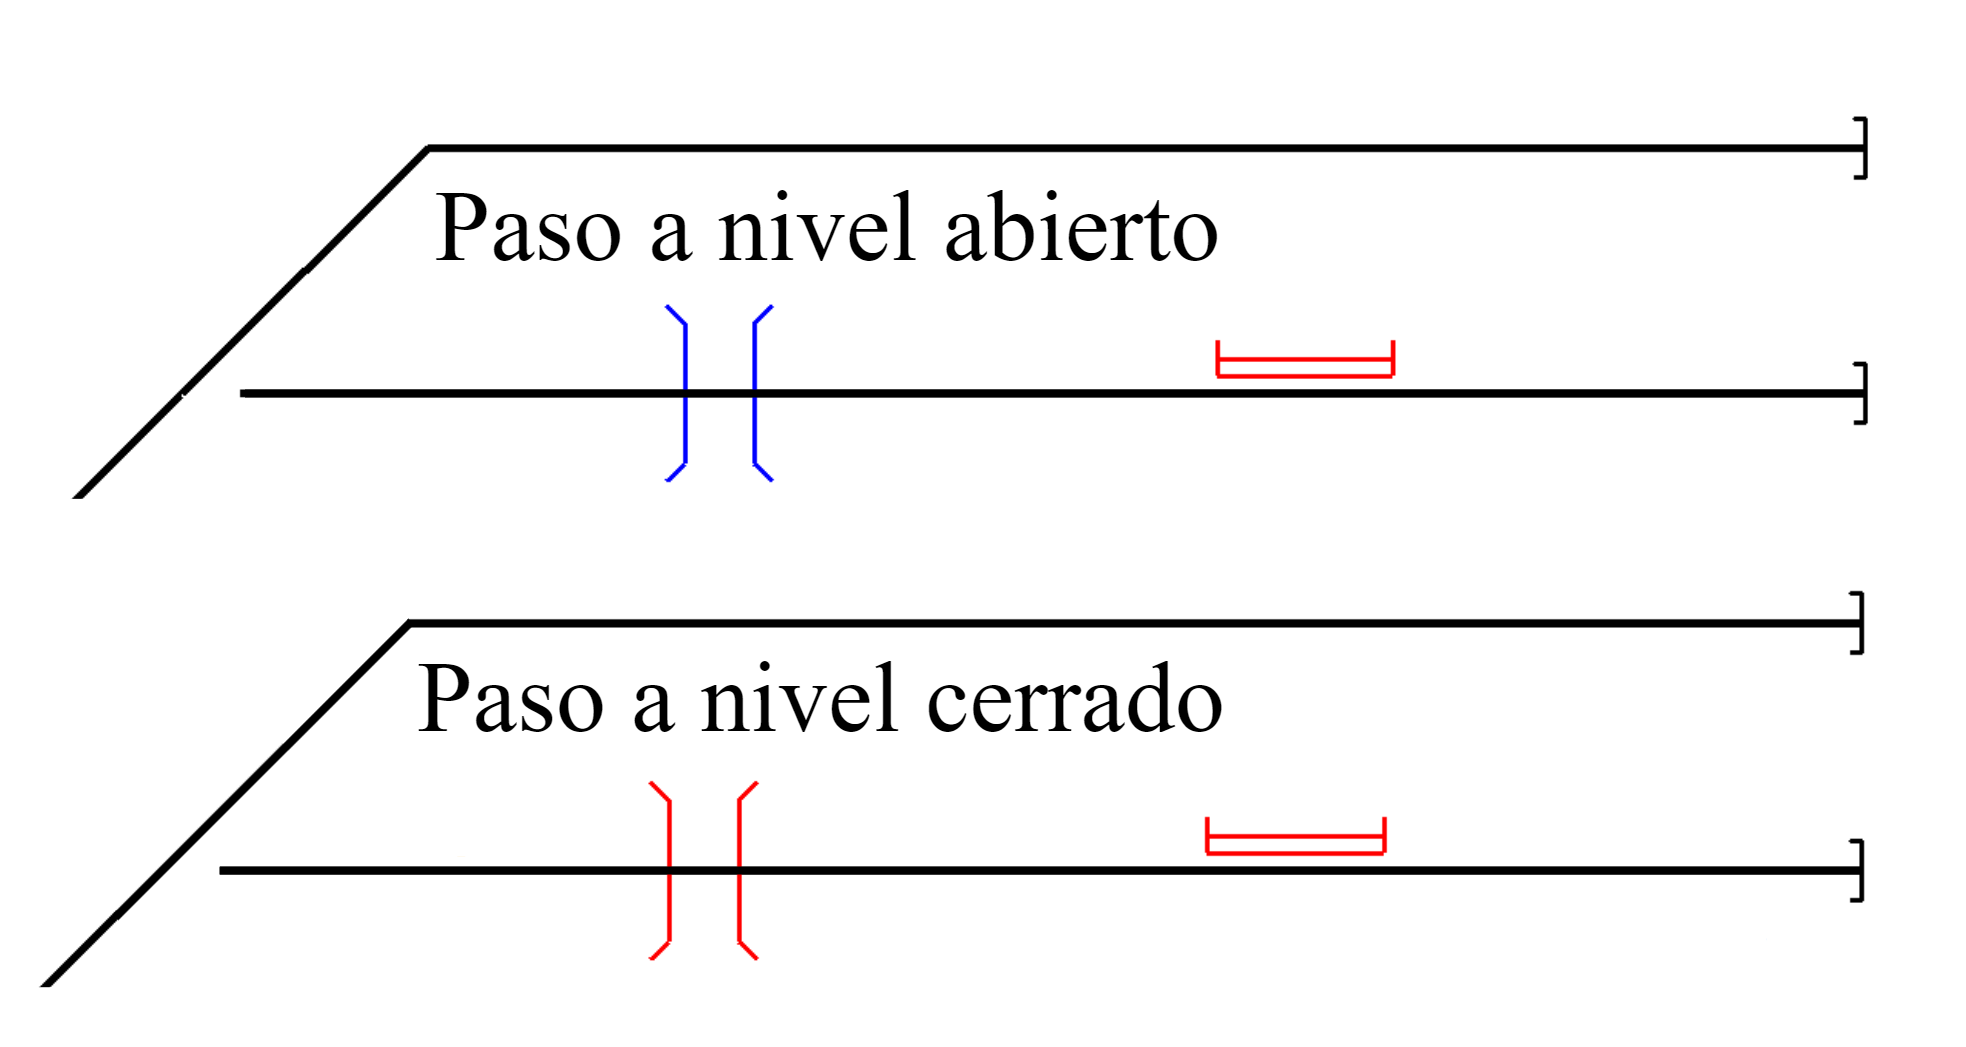
\includegraphics[width=0.7\textwidth]{AGG/images/AGG_cruce}
		\centering\caption{Representación de paso a nivel abierto (arriba) y paso a nivel cerrado (abajo) en la interfaz gráfica.}
		\label{fig:AGG_levelCrossing}
	\end{figure}
	
	Los cambio de vías simples son ilustrados en la Figura \ref{fig:AGG_switch}. El usuario puede alternar entre el estado de posición normal y posición reversa con un click sobre la unión oblicua entre la vía normal y el desvío. A diferencia de otros elementos ferroviarios interactivos que cambian su color mediante un click, los cambios de vías solamente cambian a color rojo cuando alguna de las vías que lo componen es ocupada, o a color gris si alguna de las rutas habilitadas requieren que el cambio de vías se encuentre enclavado. En este último caso, cuando el cambio de vías se encuentra enclavado, el usuario no podrá alterar la posición del mismo mediante un click.
	
	\begin{figure}[H]
		\centering
		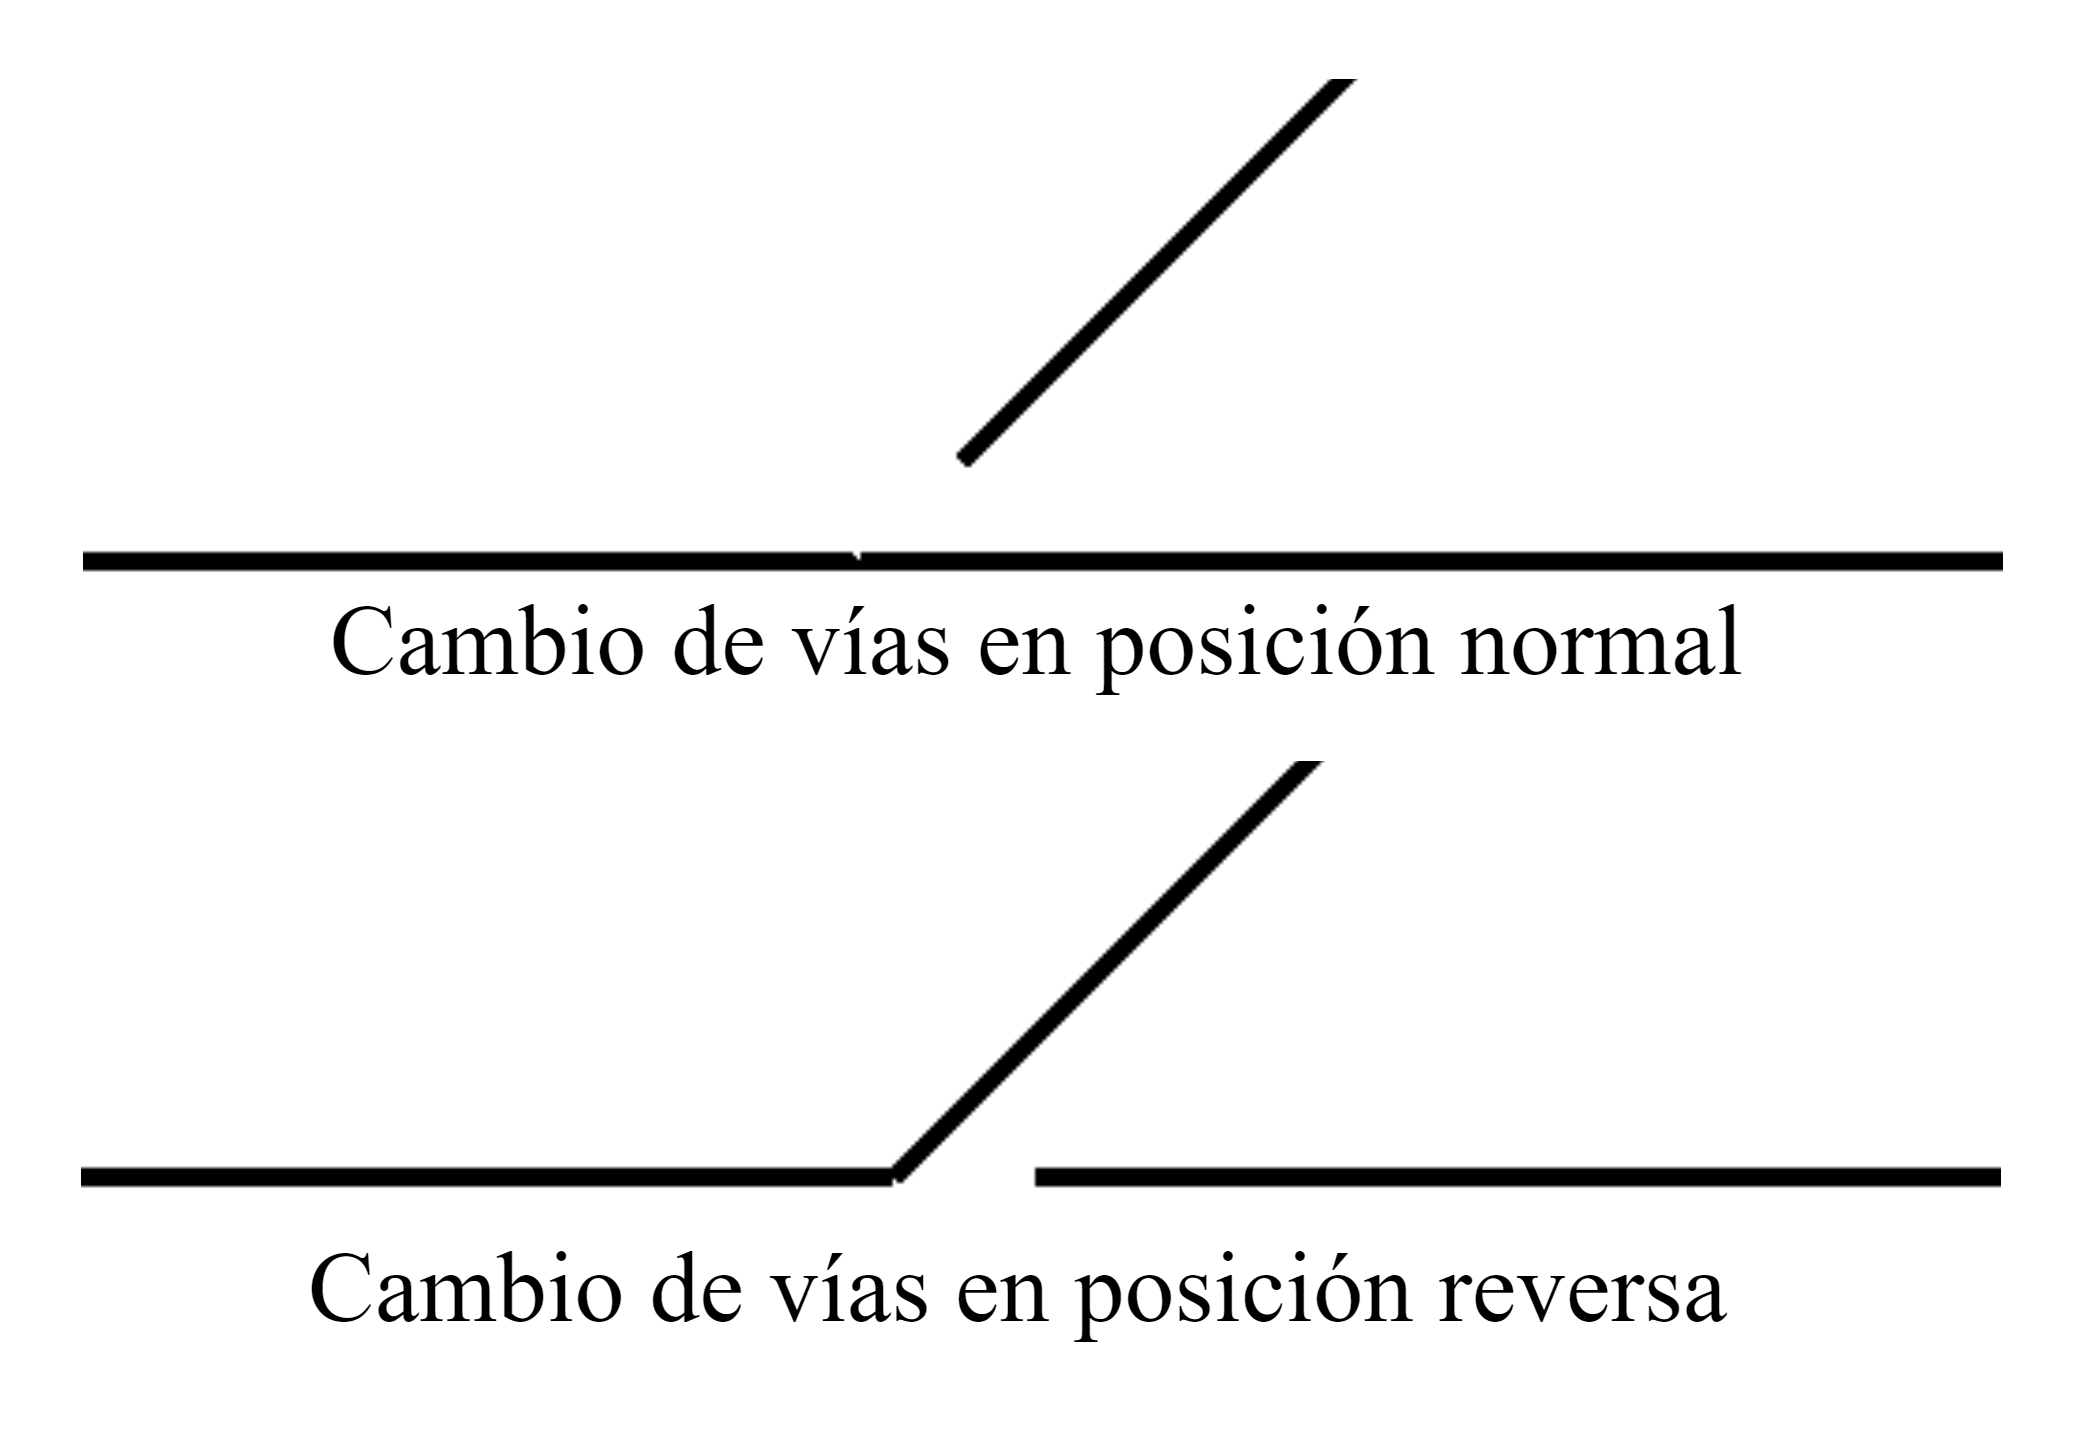
\includegraphics[width=0.6\textwidth]{AGG/images/AGG_switch}
		\centering\caption{Representación de cambio de vías simple en posición normal (arriba) y posición reverse (abajo) en la interfaz gráfica.}
		\label{fig:AGG_switch}
	\end{figure}

	Finalmente, el usuario puede solicitar o cancelar rutas de manera muy sencilla mediante un click sobre el nombre de la señal que se desea controlar. En la Figura \ref{fig:AGG_routes_1}, Figura \ref{fig:AGG_routes_2} y Figura \ref{fig:AGG_routes_3} se ilustran las tres instancias del proceso de habilitación de una ruta, junto con los distintos colores utilizados para representar los aspectos de las señales. Tal cómo fue explicado en la Sección \ref{sec:function_5}, los aspectos verde, amarillo, doble amarillo y rojo son representados por los colores verde, amarillo, naranja, y rojo, respectivamente.
	
	En la Figura \ref{fig:AGG_routes_1} el usuario aún no ha solicitado ninguna ruta ni seleccionado ninguna señal. Los nombres de las señales son de color gris oscuro y sus aspectos son determinados por el sistema de enclavamiento en base a la posición de los cambios de vías y barreras en los pasos a nivel.	
	
	\begin{figure}[H]
		\centering
		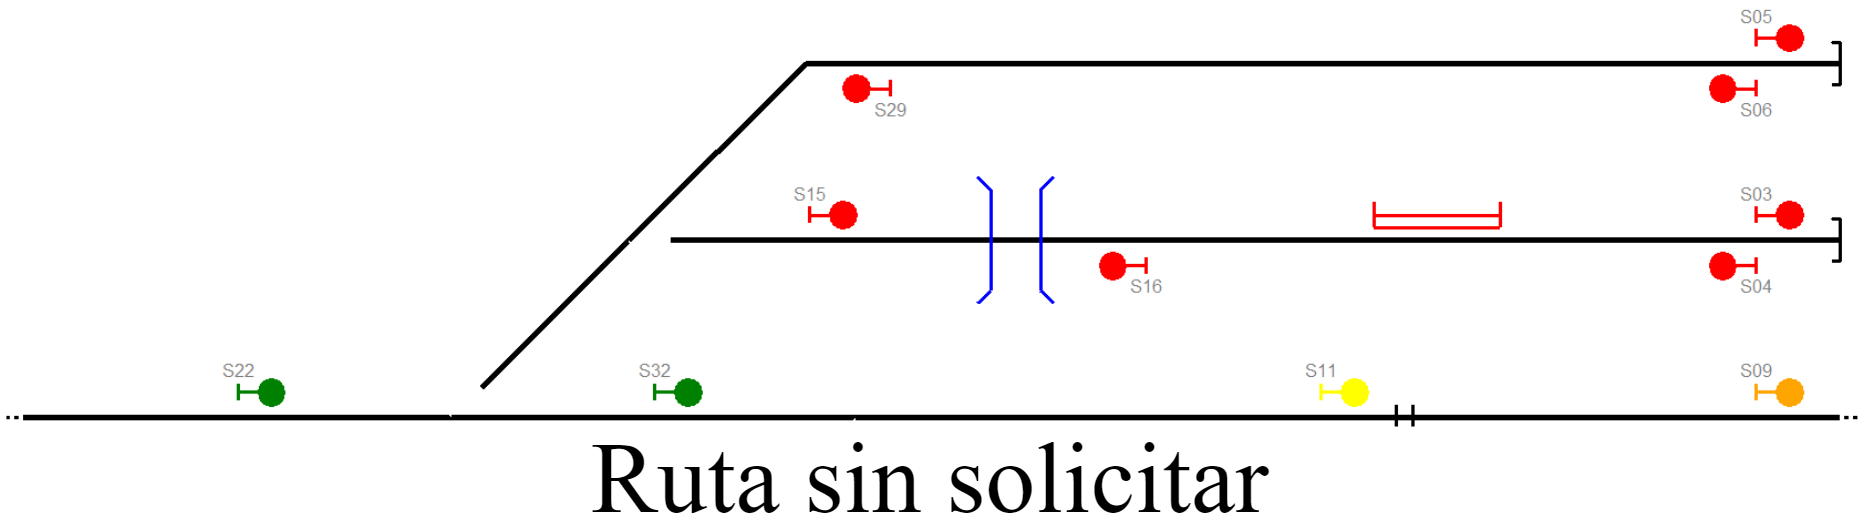
\includegraphics[width=0.85\textwidth]{AGG/images/AGG_routes_1}
		\centering\caption{Representación de ruta sin solicitar en la interfaz gráfica.}
		\label{fig:AGG_routes_1}
	\end{figure}
	
	En la Figura \ref{fig:AGG_routes_2}, el usuario seleccionó la señal S22 haciendo click sobre el nombre de la misma. Al realizar esta acción, la interfaz gráfica aún no ha enviado ninguna señal a la FPGA, pero la interfaz modifica el color del nombre de la señal a verde, para indicar que se ha elegido a la señal S22 como señal inicial de una potencial ruta. Al mismo tiempo, la interfaz cambiará el color del nombre de las potenciales señales de finalización de rutas a color rojo, en este caso: S32, S15 y S05. En cambio, todas las demás señales tendrán su nombre en color gris claro, como se observa en la Figura \ref{fig:AGG_routes_2}. 
	
	\begin{figure}[H]
		\centering
		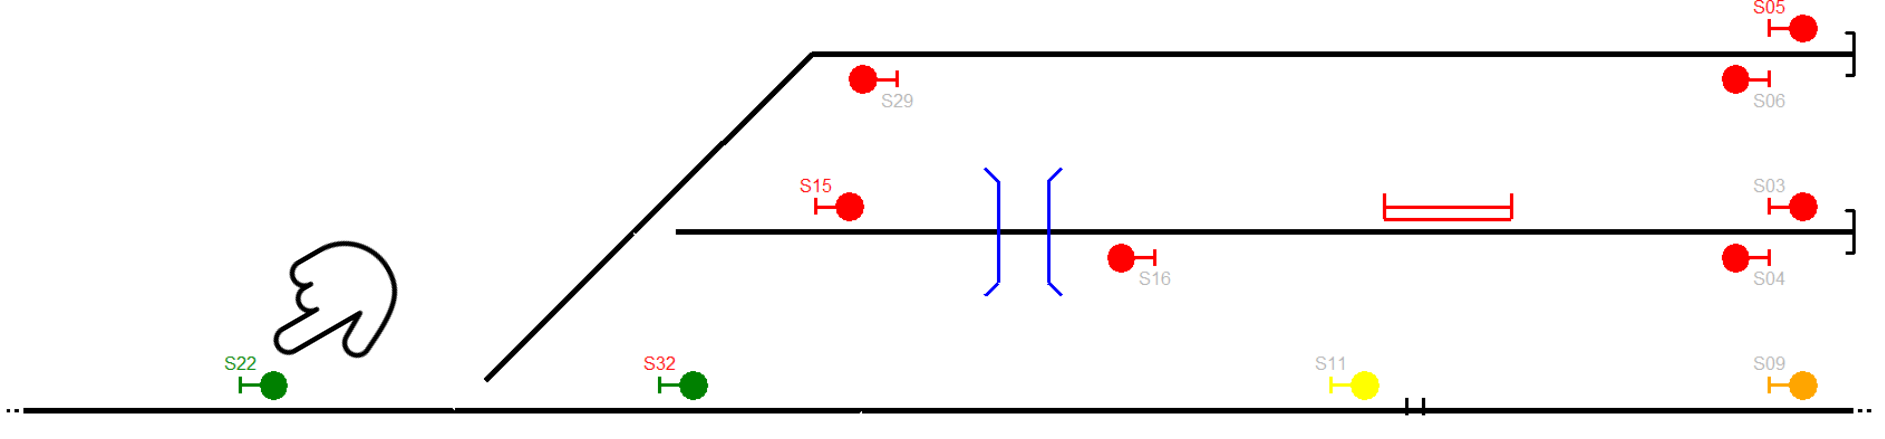
\includegraphics[width=0.85\textwidth]{AGG/images/AGG_routes_2}
		\centering\caption{Representación de solicitud de inicio de ruta en la interfaz gráfica.}
		\label{fig:AGG_routes_2}
	\end{figure}
	
	Si el usuario selecciona alguna de las potenciales señales de finalización de ruta, como por ejemplo S05, la interfaz gráfica enviará la solicitud de ruta a la FPGA. En caso de que la ruta sea aceptada, tal como se ilustra en la Figura \ref{fig:AGG_routes_3}, las vías contenidas entre la señal S22 y S05 cambiarán a color gris (enclavadas) y los cambios de vías necesarios cambiarán su posición y serán enclavados, cambiando también su color a gris, como se muestra en la Figura \ref{fig:AGG_routes_3}.
	
	\begin{figure}[H]
		\centering
		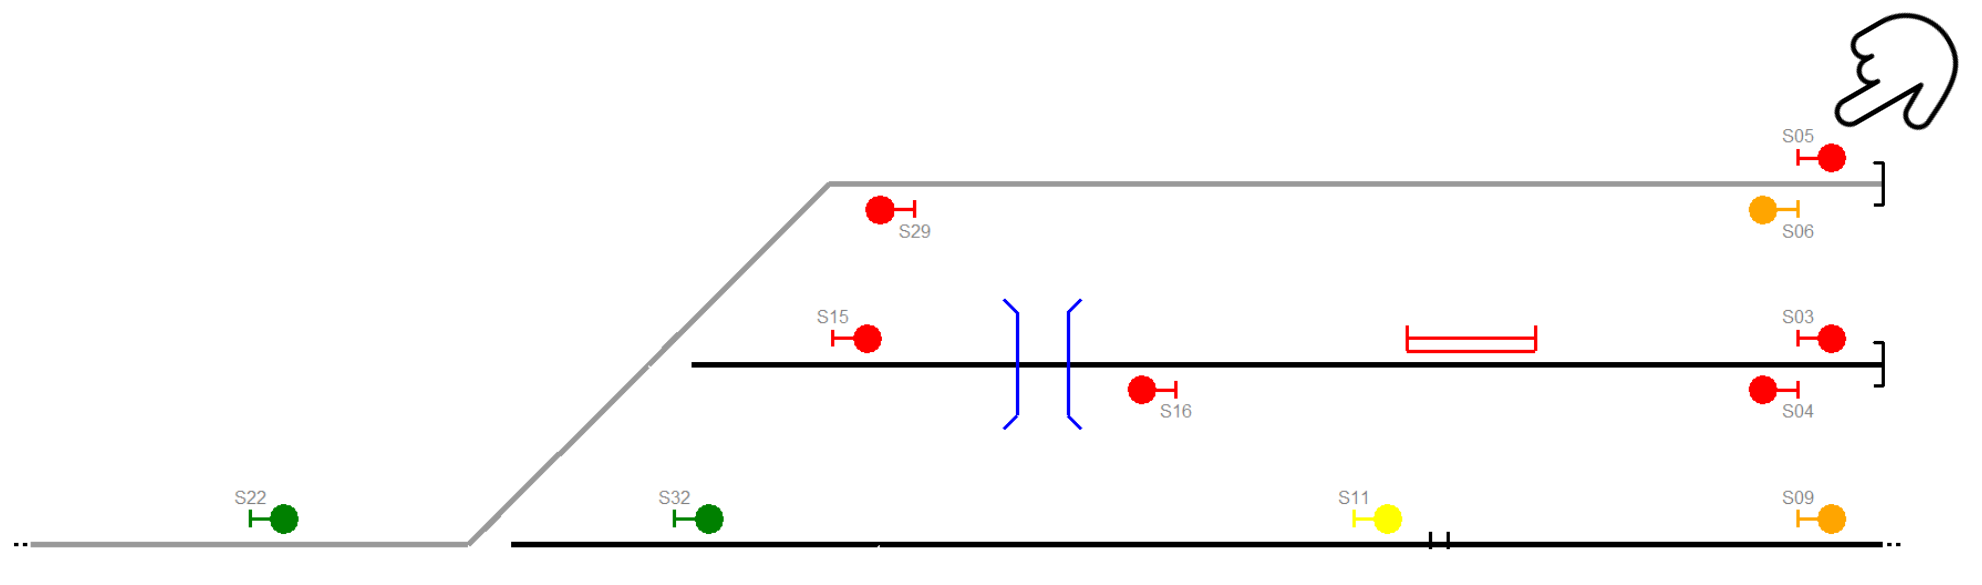
\includegraphics[width=0.85\textwidth]{AGG/images/AGG_routes_3}
		\centering\caption{Representación de ruta enclavada en la interfaz gráfica.}
		\label{fig:AGG_routes_3}
	\end{figure}
	
	El usuario podrá cancelar el pedido de una ruta que aún no fue solicitada si, en lugar de seleccionar las señales de finalización, vuelve a seleccionar la señal inicial. El usuario también puede cancelar una ruta ya habilitada si realiza un doble click sobre la señal de partida. La cancelación de la ruta será aprobada por la FPGA y removerá el enclavamiento de la infraestructura siempre y cuando sea seguro. En caso contrario, la ruta continuará habilitada.
	
	
		
	\section{Consideraciones para asegurar la convergencia del estado del sistema de enclavamientos}
	\label{sec:convergencia}
	
	Debido a que los módulos del sistema de enclavamientos reciben los datos en paralelo, el sistema no converge en un solo ciclo. A modo de ejemplo, supongamos un caso muy común en un señalamiento: dos señales A y B, tal que A depende del estado de B, por pertenecer al recubrimiento (ver Sección \ref{sec:function_5}), y ambas dependen de la trama de entrada. Al recibir la misma trama a la vez, ambas señales evolucionarán de un estado inicial a un estado final, pero la señal A lo hará utilizando la información del estado inicial de B, que ya no sería válido si B cambió de estado. Para evitar esto, el AGG compara la trama de datos enviada a la FPGA con la trama de datos recibida desde la FPGA. Si las tramas son idénticas entonces el sistema de enclavamientos ya ha alcanzado un estado de equilibrio y el AGG detendrá el envío de datos hasta que el operador altere ese equilibrio interactuando con la interfaz. En cambio, si las tramas de datos son diferentes, el AGG enviará a la FPGA la trama recibida, junto con los pedidos que el usuario pudiese haber solicitado entre ambos sucesos. De esta forma, el AGG cierra el lazo de control con la FPGA reinyectando las tramas de datos hasta que las tramas de datos converjan y se cumpla la convergencia.
	
	En la Capítulo \ref{sec:resultados} se muestran los resultados obtenidos y, cómo parte de eso, se ilustra la interfaz gráfica generada a partir de utilizar la herramienta AGG para un determinado ejemplo. En los apéndices se muestran más resultados obtenidos mediante el uso de las herramientas implementadas.

	%Los colores de cada elemento representan lo siguiente:
	
	%\begin{itemize}
	%	\item Vías: negro (libre), rojo (ocupada), gris (enclavada).
	%	\item Paso a nivel: azul (abierto), rojo (cerrado), rojo oscuro (enclavado).
	%	\item Cambio de vías: negro (libre), gris (enclavado).
	%\end{itemize}

	